\chapter{Autonomous navigation of micro-magnetic rollers on a slope$^{*}$} \footnotetext[1]{This chapter is adapted from unpublished work}
\begin{center}
\vspace*{1\baselineskip}
\textbf{Abstract}
\end{center}
Time-varying uniform magnetic field can exert torque on ferromagnetic micro particles thereby driving their rotation motions. Such rotation motions can be hydrodynamically coupled to translation motions when the micro spheres are near a boundary. Here, time-varying (spatially uniform) magnetic fields are  programmed to navigate micro spheres' rolling rolling motion on an inclined slope, showing gravitaxis behaviors(rolling either downhill or downhill). Here, a physical model is  built  to describe ferromagnetic micro particles' motions in time-varying magnetic field near a boundary. Then we introduce reverse design problem to design the optimal magnetic field for navigating different behaviors of micro particles. Some preliminary experiment results are also shown for further investigation. 
\section{Introduction}
Living cells or bacteria show the fantastic ability of navigation called chemotaxis\autocite{alon1999robustness,adler1975chemotaxis}. The chemotactic microorganism can trace the very limited information in  a complex micro noisy environment for the food source or suitable living space\autocite{keller1971model}. This kind of navigation behavior in the living system is also highly desirable in synthetic micro swimmers or active matter systems \autocite{patteson2016active}. Only with efficient and accurate navigation behaviors in a complex environment, synthetic micro swimmers can extend their engineering application  such as drug delivery and surgery\autocite{de2017micromotor,xu2018sperm}. Although lots of synthetic  micro swimmers can do autonomous directed motion \autocite{yan2016reconfiguring,dou2016directed,lee2019directed,baker2019shape}, their motions are biased by  external field or inherent asymmetry instead of information from environment. Thereby, it is essential to introduce new strategies for micro swimmers so that micro swimmers can interact with the environment and show navigation behaviors.  

The suffix "-taxis" refers to the motion following a physical or chemical properties gradient. Recently, different experimental or theoretical research has been reported to make "taxis" synthetic microswimmers. Phototaxis particles can see the gradient of light due to the local thermal gradient near the particle\autocite{yu2019phototaxis,dai2016programmable,lozano2016phototaxis,chen2017light}; gravitaxis swimmers can swim against the gravity \autocite{campbell2013gravitaxis,ten2014gravitaxis}; rheotaxis swimmers can orient their direction autonomously against the fluid flow\autocite{Palacci2015,ren2017rheotaxis,brosseau2019relating}; bio-mimic chemotaxis swimmers can sense the local gradient of species and move towards the source or drain of chemicals\autocite{dou2019autonomous}; visoctaxis particles can swim towards the fluid regions of higher or lower viscosity\autocite{liebchen2018viscotaxis}. However, these approaches depend on the precise fabrication of microswimmers.
These reports all use particles of particular shapes or components. Different navigation directions can only be achieved by redesigning the particles, which is a complex and non-efficient process. Less research has been reported to navigate an isotropic particle's taxis behaviors. A more programmable and tangible mechanism is needed to navigate a large amount of particles autonomously \autocite{dou2019autonomous}.

Here, we propose a new gravitaxis mechanism that uses a programmed time-varying magnetic field on isotropic magnetic microspheres placed on an inclined surface. Microspheres in fluid rolling on a surface can couple the rotational motion to translation motion via hydrodynamics\autocite{galvin2001time,rashidi2016theoretical}. Magnetic micro spheres with permanent magnetic dipole  can response to the external  magnetic showing different rolling dynamics \autocite{helgesen2019propulsion,helgesen2018magnetic}.
The external magnetic field provides a rich programmed design space to control the dynamics of magnetic rollers.
In this chapter, we show how to program the external magnetic field exerted on  micro rollers to achieve autonomous gravitaxis behaviors on an inclined slope. First, we describe a physical model to simulate the motions of magnetic rollers on an inclined surface subject to external magnetic field. Then we explore the design parameters space for the magnetic field  and optimize the field leading to desired motions of  micro rollers. At the end of this chapter, we show some preliminary experimental results as well as a challenge discussion for future investigation in this system. 

\section{Model of  magnetic microrollers}
\begin{figure}[p]
\centering
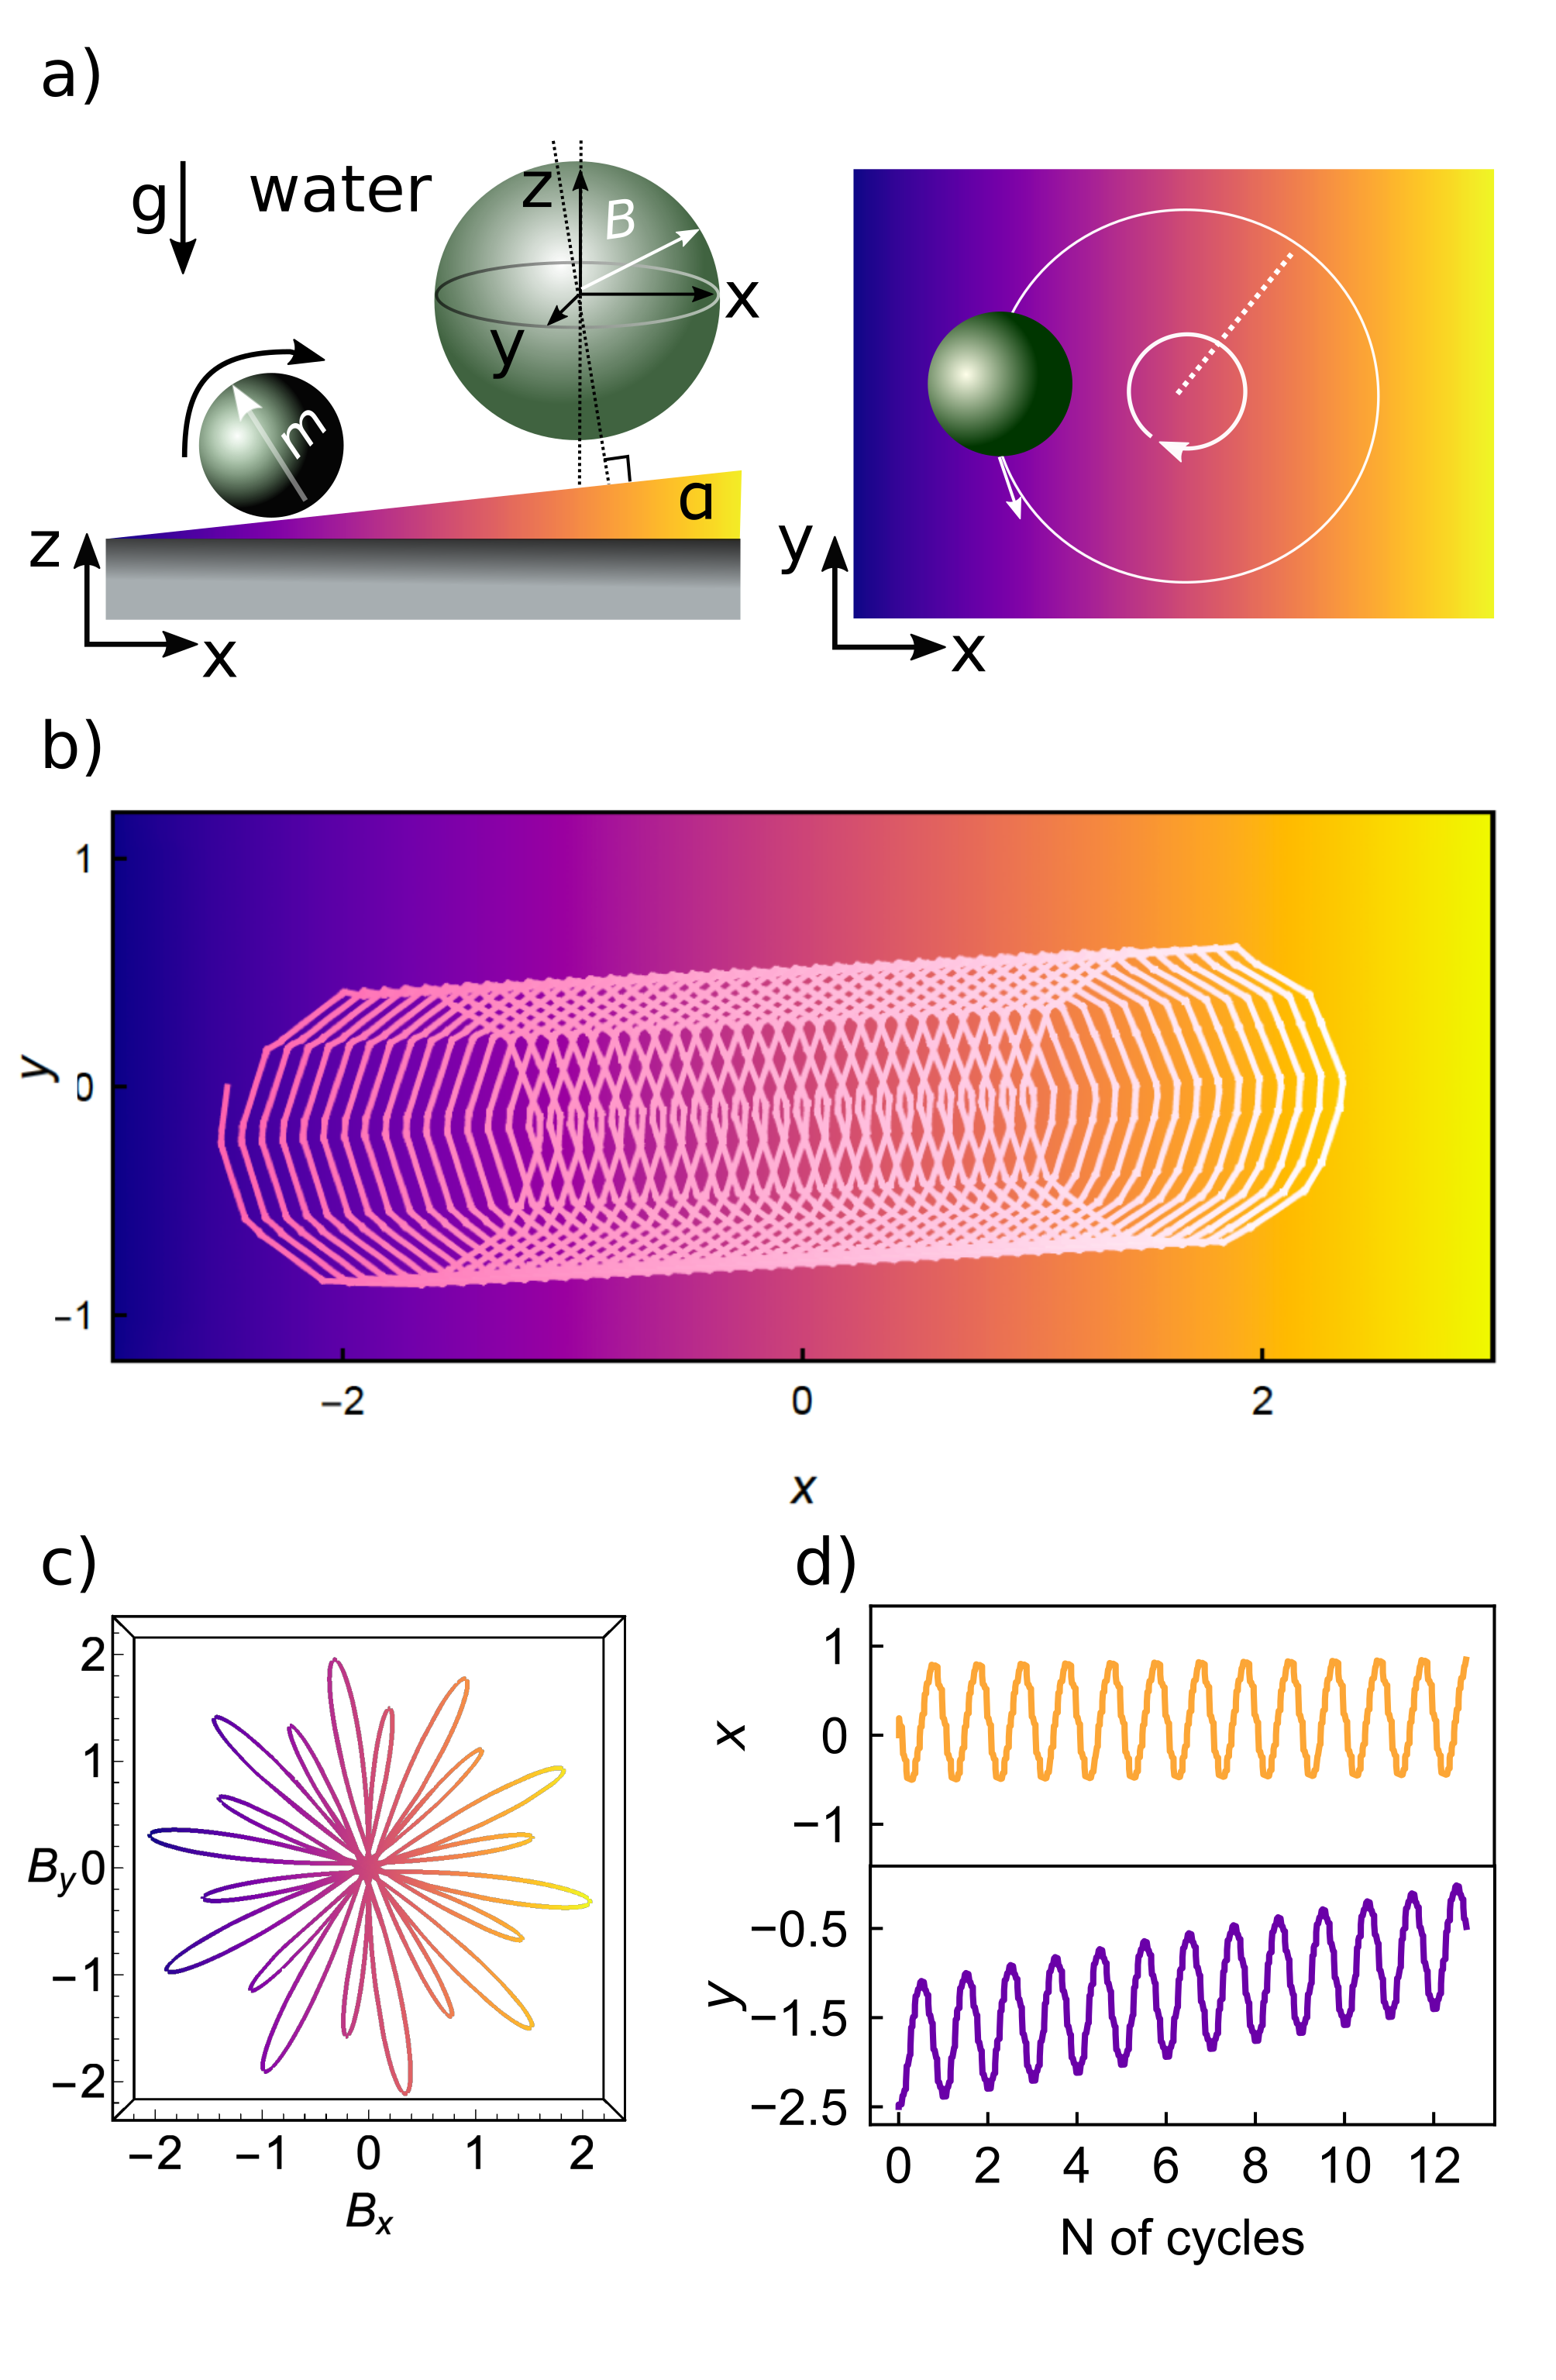
\includegraphics[width=9cm]{figures/5_1.png}
\caption{ (a) Schematic illustration of a magnetic micro particle with radius$a$, magnetic moment$m$ rolling on an $\alpha$ angle inclined surface subject to a three-dimensional magnetic field$B$. Plasma color is used to represent the height change of the surface. The left figure shows the side view while the right figure shows the top view. (b) A simulated trajectory (from left to right) with gravitaxis behaviors on an inclined surface with an angle of $10$ degree. (c) The applied magnetic field that leads to the trajectory in figure(b). (d) Plot of the particle's position in x and y direction versus time.}
\label{fig:5.1}
\end{figure}
We consider a magnetic sphere with radius $a$ and permanent magnetic moment $\ve{m}$ moving through a viscous fluid at a fixed height above a solid plane under the influence of a time-varying magnetic field $\ve{B}(t)$. (as shown in Fig. 5.1a and 5.2a) In a uniform field, the particle experiences a magnetic torque, $\ve{L}_{\m}=\ve{m}\times\ve{B}(t)$, but no magnetic force, $\ve{F}_{\m}=0$. In the absence of inertial effects (i.e., at low Reynolds number), the magnetic force and torque on the particle are balanced by the hydrodynamic force and torque, which are linearly related to the particle's linear velocity $\ve{U}$ and angular velocity $\ve{\Omega}$ noted as
\begin{equation}
    \begin{bmatrix} \ve{F}_{\m} \\ \ve{L}_{\m} \end{bmatrix} = \begin{bmatrix} \ve{A} & \ve{\tilde{B}} \\ \ve{B} & \ve{C} \end{bmatrix}  \cdot \begin{bmatrix} \ve{U} \\ \ve{\Omega} \end{bmatrix} \label{eq:dynamics}
\end{equation}
where $\ve{A}$, $\ve{B}$, $\ve{\tilde{B}}$, and $\ve{C}$ are components of the hydrodynamic resistance tensor.  For a solid sphere above a solid plane normal to the $z$-direction, the components of the resistance tensor have the form


\begin{equation}
{\scriptstyle
    \ve{A} &=  6\pi \eta a \begin{bmatrix} 
        Y_A & \cdot & \cdot \\
        \cdot & Y_A & \cdot \\
        \cdot & \cdot & X_A  \end{bmatrix}, \quad 
    \ve{B}=-\ve{\tilde{B}}&= 6\pi \eta a^2 \begin{bmatrix} 
        \cdot & Y_B & \cdot \\
        -Y_B & \cdot & \cdot \\
        \cdot & \cdot & \cdot  \end{bmatrix}, \quad 
    \ve{C} =- 6\pi \eta a^3 \begin{bmatrix} 
        Y_C & \cdot & \cdot \\
        \cdot & Y_C & \cdot \\
        \cdot & \cdot & X_C  \end{bmatrix} 
    }
\end{equation}
where $\eta$ is the fluid viscosity. The coefficients $Y_A$ and $Y_B$ describe, respectively, the dimensionless force and torque on a sphere translating parallel to a solid planar surface\autocite{ONeill1964a}. The coefficient $Y_C$ describes the torque on a sphere rotating about an axis parallel to the surface\autocite{Dean1963}. The coefficient $X_A$ describes the force on a sphere translating perpendicular to the surface \autocite{Brenner1961a}.  Finally, $X_C$ describes the torque on a sphere rotating about an axis perpendicular to a the surface \autocite{Jeffrey1915}. These coefficients depend only on the surface separation $\delta$ scaled by the particle radius $a$.

Substituting the above expressions for the resistance tensor, the linear velocity $\ve{U}$ and angular velocity $\ve{\Omega}$ can be expressed explicitly in terms of the magnetic torque. The dynamics imply that the particle velocity normal to the planar substrate is identically zero (i.e., $U_z=0$). We, therefore, assume that the surface separation $\delta$ and the resistance coefficients are constant throughout the particle's dynamics. For a sphere on an inclined surface with angle$\alpha$, we can change the coordinate from a world frame to the particle frame as shown in Fig. 5.2a, making the rollers  on a horizontal surface. To simplicity, we assume the gravity's influence is negligible with $mg\times a<< m\time B(t)$. The surface force $F_s$ is modeled to balance any force normal to the surface that will not influence the dynamics of particles. The magnetic field the frame of the particle is expressed as
\begin{equation}
    B'(t)=R_y(\alpha) B(t) 
\end{equation}
Where $R_y(\alpha) $ is the rotation matrix around y axis.  The dynamics of particles angular and translational velocity are solved numerically to determine the particle position $\ve{x}_{\p}(t)$ and its orientation parameterized by the unit quaternion $\ve{q}(t)=[q_0,q_1,q_2,q_3]^T$\autocite{diebel2006representing} (See the details of numerical simulation of three dimension roller in reference\autocite{fei2019magneto}). 
\begin{figure}[p]
\centering
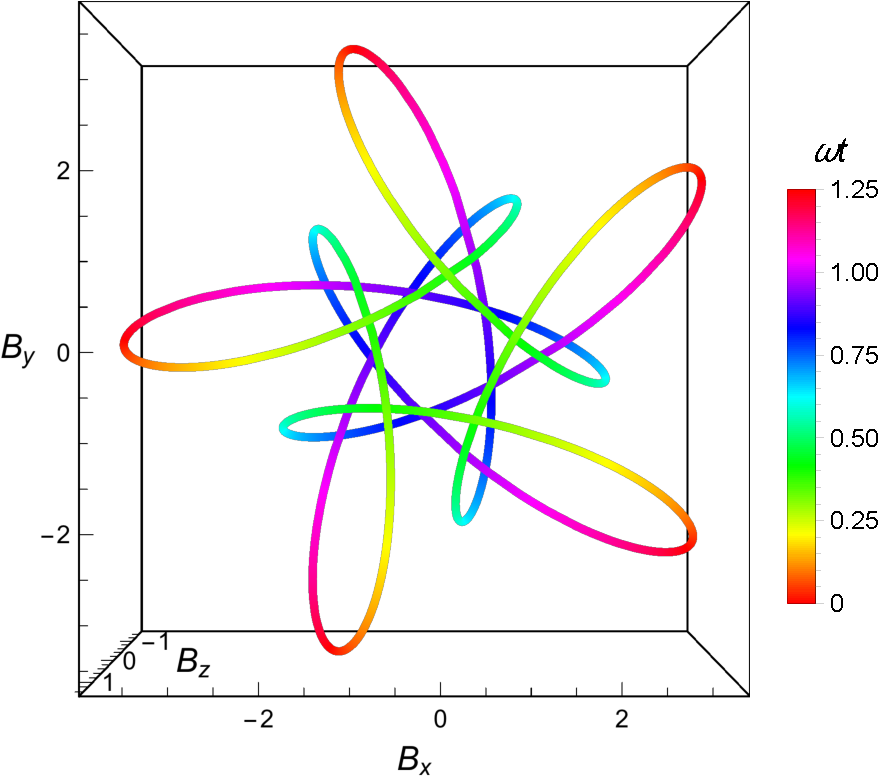
\includegraphics[width=9cm]{figures/5_2.pdf}
\caption{ (a) Left: The force balance on the magnetic roller on an inclined surface. $L_m$ is the magnetic torque. $L_H$ is Hydrodynamics torque. The gravity force$mg$ and hydrodynamics force$F_H$ are balanced by surface force$F_S$   right: transform from world frame to particle frame. Particles have three degrees of freedom for rotation. (b) The design process for the magnetic field. The physical model can forward simulate the dynamics of rollers on the inclined surface. Moreover, the simulation results can inversely guide the design of magnetic field by properly defining the target function.}
\label{fig:5.2}
\end{figure}
 \section{Design the Magnetic Field}
 The desired magnetic field should be periodic that lead no net motions from cycle to cycle for particles on a horizontal surface and navigate particles gravitaxis motions on an inclined surface.
 We consider periodic magnetic fields $\ve{B}(t)$ with a fundamental frequency $\omega$ and $N$ harmonics
\begin{equation}
    \ve{B}(t) = \tfrac{1}{2} \ve{a}_0 + \sum_{n=1}^N \ve{a}_n \cos(n\omega t) + \ve{b}_n \sin(n\omega t)
\end{equation}
where $\ve{a}_n$ and $\ve{b}_n$ are constant vectors. This $6N+3$ dimensional design space is constrained by additional requirement that the field have $m$-fold rotational symmetry about the $z$-axis
\begin{equation}
    R_z(\varphi_m) \ve{B}(\omega t) = \ve{B}(\omega t - \varphi_m) \label{eq:symmetry}
\end{equation}
where $\varphi_m=2\pi/m$ for positive integer $m\geq 3$, and $R_z(\varphi)$ is the rotation matrix about the $z$-axis.
For $n=0$, equation (\ref{eq:symmetry}) implies that $\ve{a}_0 = a_0 \ve{e}_z$. For $n\geq1$, equation (\ref{eq:symmetry}) has terms like $\cos(n \omega t)$ and $\sin(n\omega t)$, which can be collected to give six linear equations for the six coefficients 
\begin{equation}
    \begin{bmatrix} 
    R_z(\varphi_m) - I \cos(n\varphi_m) & I \sin(n \varphi_m) \\
    -I \sin(n \varphi_m) & R_z(\varphi_m) - I \cos(n\varphi_m)
    \end{bmatrix} 
    \begin{bmatrix} \ve{a}_n \\ \ve{b}_n \end{bmatrix} = 0
\end{equation}
where $I$ is the identity matrix.  Importantly, these equations six equations are not always independent of each other, in which case there exists a null space of non-trivial solutions for the coefficients $\ve{a}_n$ and $\ve{b}_n$.  For example, when the field has $m$ fold rotation symmetry, the $n=1$ harmonic has coefficients of the form 
\begin{equation}
    \begin{bmatrix} \ve{a}_1 \\ \ve{b}_1 \end{bmatrix} = c_1 \begin{bmatrix} 1\\0\\0\\0\\1\\0 \end{bmatrix} + d_1 \begin{bmatrix} 0\\1\\0\\-1\\0\\0 \end{bmatrix}
\end{equation}
where $c_1$ and $d_1$ are arbitary coefficients. For a given order of rotational symmetry $m$, non-trivial solutions exists for $n=1$, $n=k m-1$, $n=k m$, and $n=k m + 1$  where $k= 1,2,\dots$ is a positive integer. For $m$-fold rotational symmetry, the corresponding null space is given by
\begin{align}
    \quad \begin{bmatrix} \ve{a}_{n} \\ \ve{b}_{n} \end{bmatrix} &= c_{n} \begin{bmatrix} 0\\0\\1\\0\\0\\0 \end{bmatrix} + d_{n} \begin{bmatrix} 0\\0\\0\\0\\0\\1 \end{bmatrix} \quad \text{for} \quad n=km
    \\
    \quad \begin{bmatrix} \ve{a}_{n} \\ \ve{b}_{n} \end{bmatrix} &= c_{n} \begin{bmatrix} 1\\0\\0\\0\\\pm1\\0 \end{bmatrix} + d_{n} \begin{bmatrix} 0\\1\\0\\\mp1\\0\\0 \end{bmatrix} \quad \text{for} \quad n=km \pm 1
\end{align}
for positive integers $k$ and $m\geq3$. To limit the size of our design space, we fix the number of higher harmonics to $N=m+1$. In this way, the full $6N+3$ dimensional design space is reduced to only 9 dimensions (namely, $a_0$, $c_1$, $d_1$ $c_{m-1}$, $d_{m-1}$ $c_{m}$, $d_{m}$, $c_{m+1}$, and $d_{m+1}$). As the phase of the driving field is not important, we set $d_1=0$ without loss of generality.  Moreover, as the field has rotational symmetry about the $z$ axis, rotation of the field about that axis by any angle is not important; we can therefore set $d_{m-1}=0$ without loss of generality.  Fig. 5.1c illustrates one possible magnetic field with $m=10$ fold symmetry.

To design a magnetic field, we use our model to numerically simulate our particles' trajectories on the slope. The physical model works as a black box model (shown as Fig. 5.2b) with input as variables, $a_0$, $c_1$, $c_{m-1}$, $c_{m}$, $d_{m}$, $c_{m+1}$, and $d_{m+1}$ (to simplify the notation, we re-denote the input as $\vec{v}=$ $v_1$,$v_2$,$v_3$,$v_4$,$v_5$,$v_6$,$v_7$  ). The output of the black-box function is the dynamics of particles. In order to achieve the desired gravitaxis motion, we defined the target function as,
\begin{equation}
    f(\vec{v})=|\frac{\delta y}{\delta x}| sign(\delat x)
\end{equation}
where $\delta x$ and $\delta y$ are the net displacement of particles after one period of  time-varying magnetic field $B(t)$ parameterized with $\vec{v}$.
The black-box optimization algorithm is applied to minimize the target function\autocite{dou2019autonomous}. Minimization of target function $f(\vec{v})$ is trying to maximum the gavitaxis motion uphill while reducing the motion perpendicular to the gravity as much as possible. The design process is shown in Fig. 5.2b and the optimized field with the desired trajectory is plotted in Fig. 5.1b and Fig. 5.1c.


 
\section{Discussions}
In addition to optimizing the magnetic field, we also explore how the navigation dynamics depend on different physical parameters in the system. We select 20 optimized fields and numerically study the influence of distance from the particle to surface $\delta$, the number of  rotational symmetry number $N$, inclined surface angle $\alpha$ and  minimum frequency of system  $\omega$. The results are plotted in Fig. 5.3b to Fig 5.3e. As shown in Fig. 5.3b, the navigation displacement $\delta y/a$ decreases while $\delta$ increases. The physical explanation for this is that coupling between rotation and translation motion gets weaker for the larger distance between particle and surface. We also found that the navigation displacement is increasing as we increase the   number of  rotational symmetry number $N$, inclined surface angle $\alpha$ and  minimum frequency of system  $\omega$, which can be used to increase the navigation velocity. The physical explanation between the navigation behaviors and these parameters is still uncleared and need further theoretical study. 



\begin{figure}[p]
\centering
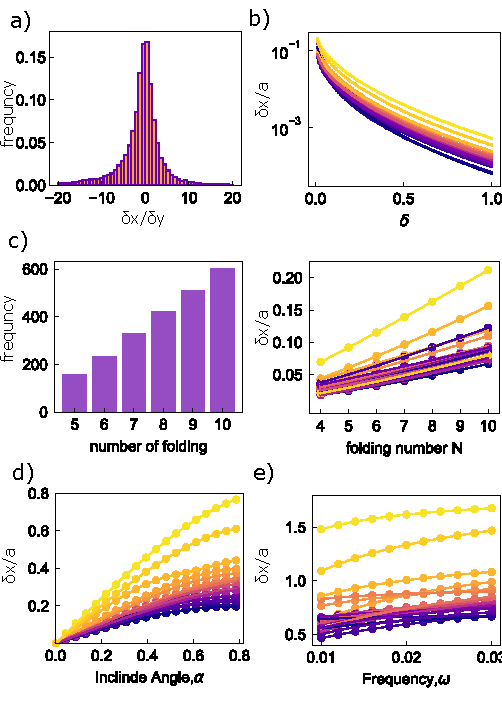
\includegraphics[width=9cm]{figures/5_5.pdf}
\caption{(a) Distribution of the navigation directions in the statistical study; Navigation behaviors depend on the physical properties. (b) The distance between spheres and surface $\sigma$, (c) the number of summery $N$, (d) the angle of slope surface $\alpha$, and (e) minimum frequency of system  $\omega$. }
\label{fig:5.5}
\end{figure}


We also did a statistical study on how the design variables $\vec{v}$ influence the  navigation behaviors for particles. 100k random data points were generated first in seven dimensions for $\vec{v}$ with the Latin-hypercube method\autocite{park1994optimal}. The target function is evaluated 100k times via paralleling computing. Fig. 5.4 plots the pair plot of the statistical study result. We plot KDE (kernel density estimate) distribution plot for each variable and plot the correlation contour plot between different parameters. The right upper part plot the date corresponding to the navigation to uphills ($\delta x>0$) while the left bottom part plot the date corresponding to the navigation to downhills ($\delta x<0$). From Fig. 5.4, apparently, the data pattern for uphill and downhill motions are different. From the KDE plot, the parameters leading to uphill motions are distributed around mean value $\vec{v}=[0.5,0.5,0.5,0,0,0.5,0.5]$, which tries to squeeze the magnetic field shape in z-direction making the magnetic field  very flat. This founding from statistics agrees with our optimization results. As comparison, the parameters leading to downhill motions are distribute around mean value $\vec{v}=[0,0,0,1,1,0,0]$, which try to 
stretch the magnetic field shape in the z-direction.
 
 
 \begin{figure}[p]
\centering
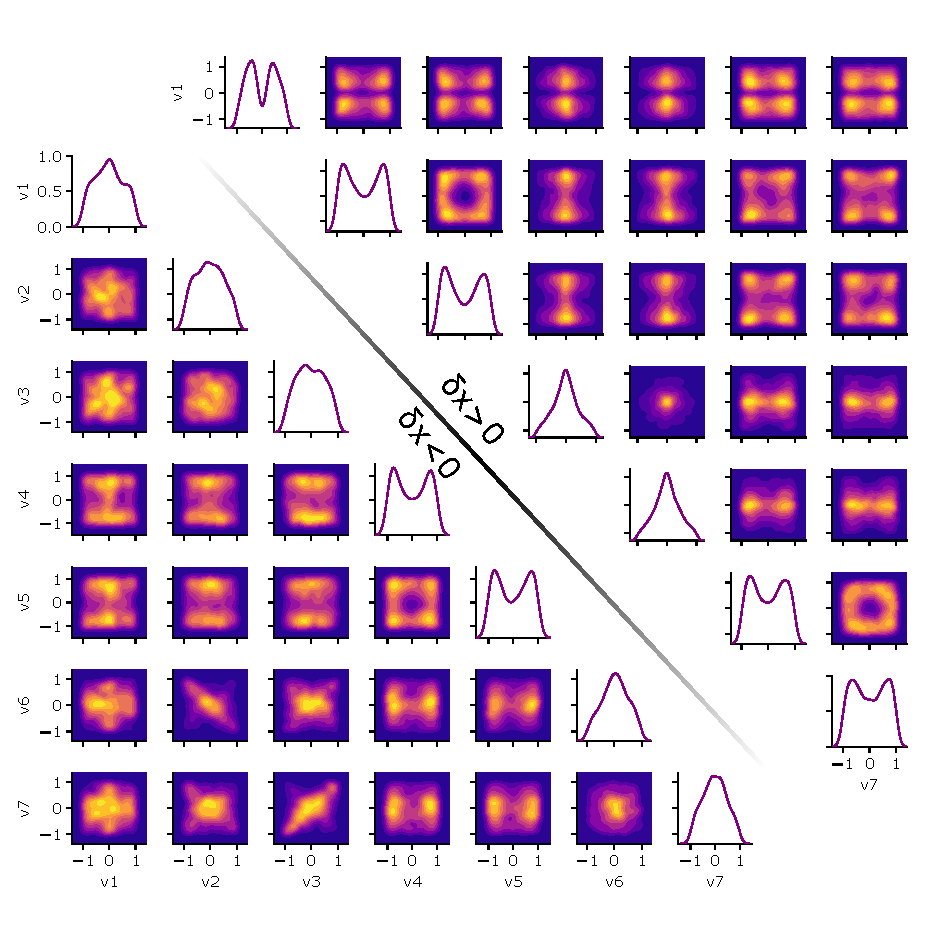
\includegraphics[width=16cm]{figures/5_4.pdf}
\caption{ Statistical study on the designed magnetic field and navigation behaviors with 100k simulations. The pair plot shows the distribution of parameters$\vec{v}$ and correlations between each design parameter for negative/positive gravitaxis separately.}
\label{fig:1}
\end{figure}
 
 
 
 \section{Preliminary experiment results and challenge}
 The experimental setup is adapted from our group's previous paper\autocite{fei2018magneto, fei2019magneto}. A 3-dimensional time-varying magnetic field is generated with a three-axis electric magnetic coil mounted on the microscope. The orientation of magnetic field is controlled by the wave function in $x$, $y$, and $z$ direction. The magnitude of the magnetic field is controlled by the current. The field can be rotated by multiply a 3-d rotational matrix. 3D printed  surfaces with slope angles from $5^o$ to  $20^o$ are put under microscope to generate gravity field. We use one optimized magnetic field (10 symmetry number with the flat shape  squeezing in z-direction) to apply torque on the experimental ferromagnetic particles. The results are shown in Fig. 5.5. When the magnetic field is flat without rotation along the y-axis, the particles are just following the periodic magnetic field showing no directed motion. Interestingly, as we rotate the magnetic field around $20$ degree, and apply the same kind of periodic field, the particles began to show a very clear directed motion from left to right as shown in Fig. 5.5b. However, this directed motion is different from the simulation result. The mismatching results between experimental results and simulation happens a lot, which seems a very big challenge. 
 
 The reason for the incorrect prediction results in our model for real experiments may be caused by inadequate physics. There are lots of assumptions in our model to simplify the questions, which may not be accurate. For example, in our model,  we assume the distance $\delta$ between the particle and surface is constant. Considering the constantly changing rotation direction of particles and the surface force from the slope, this constant surface separation assumption may not be accurate. Fig. 5.3b has shown how $\delta$ can affect the dynamics of rollers. The induced magnetic dipole inside the particle with a high frequency external magnetic field can also add new force and dynamics, leading different trajectories.
 So if our model wants to capture the real experiment behaviors, a more precise and detailed physics model should be proposed to  simulate the dynamics of micro rollers. Another reason of this mismatch between experiment and simulation may be the noise of the system. There are lots of noises in the experiment system  such as the real magnitude and direction of the magnetic field compared to our perfect simulation results. Our optimized algorithm only finds a good  "point" on a very noise solution space instead of a region. If some parameters are really sensitive (for example, changing 1$\%$ amount of this parameter will lead to totally different results), it is not surprising that noise in the experiment can lead to different results from the simulation. We can make our experiment setting better by using more accurate equipment to reduce the noise. Alternatively, we can re-program the optimization algorithm to let it find the best optimized results in a region with some noise instead of a single point. However, if the optimized  surface or blob is much harder to achieve than the optimized point, we can use other shapes in other navigation systems. Non-spherical shapes have very different hydrodynamic resistance tensor\autocite{brooks2018shape} so that particular shape may easier to have the navigation behaviors. Another very promising approach is to use real experiment results as the output of blackbox function and optimize the parameters dynamically with the real experiment output. This will need the automation of experiment process that can automate apply field, capture and analyze  videos to generate a large amount of real experiment data\autocite{oulmas20183d}.

 \begin{figure}[p]
\centering
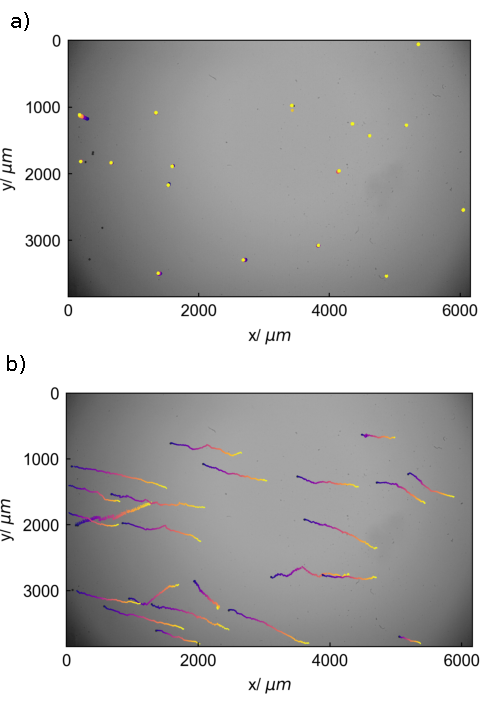
\includegraphics[width=9cm]{figures/5_6.pdf}
\caption{An experiment showing navigation motions of magnetic rollers (a) Particles with no navigated motion on a planner surface doing periodic closed trajectory motion.  (b) Particles with navigated motion driven by a inclined magnetic field.}
\label{fig:1}
\end{figure}
